\subsection{Vorhergegangene Arbeit}

\

\begin{wrapfigure}{l}{0.45\textwidth}
    % \begin{figure}[h]
     \vspace{-\baselineskip}
         \centering
         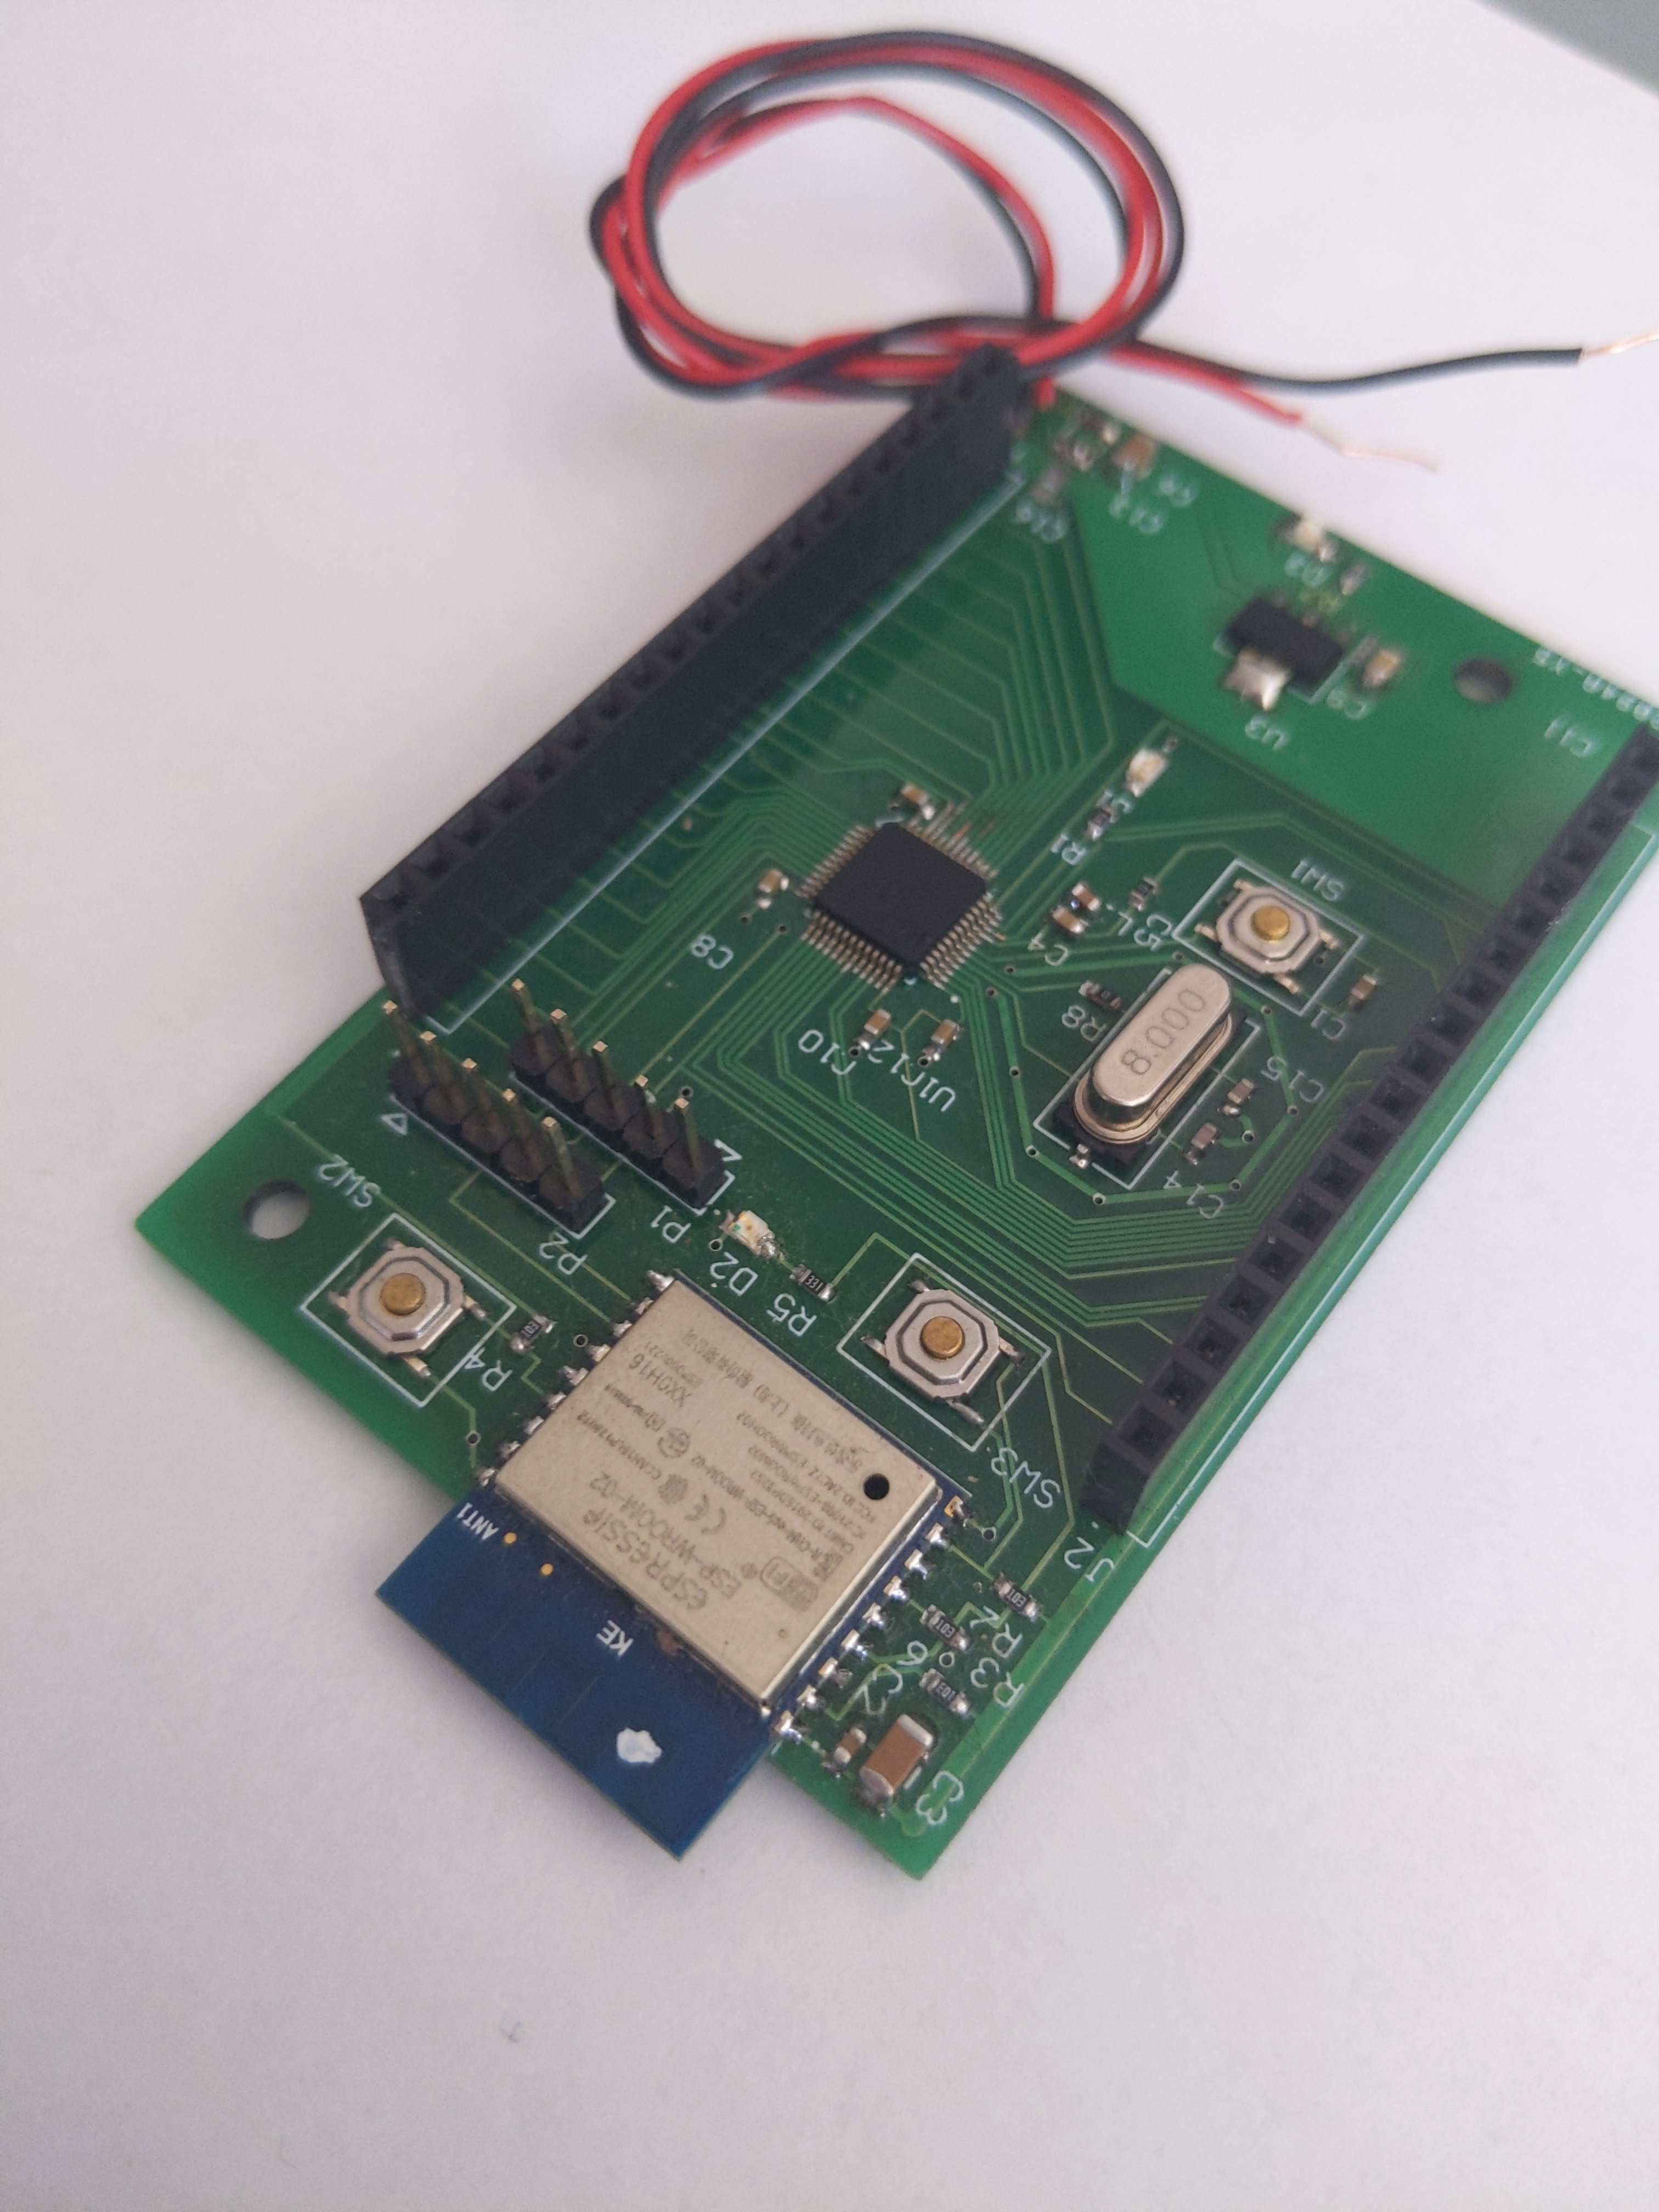
\includegraphics[scale=0.05]{Pictures/assembled.jpg}
         \caption{\textit{IoT-Gateway \citep{IoTGateway}}}
         \label{img:IoT-Gateway}
    % \end{figure}
 \end{wrapfigure}

In der vorhergegangenen Arbeit \textit{Entwicklung eines IoT-Gateways \citep{IoTGateway}} wurde eine Platine, zu sehen in Abb. \ref{img:IoT-Gateway}, 
entwickelt, welche die Grundlage dieser Arbeit bildet. 

\smallskip


Die Platine verfügt über zwei \ac{uC}. Einer der Prozessoren, genauer ein \textit{STM32F103C8} ist für das auslesen von Messwerten und die
verarbeitung dieser Zuständig, währen der andere Prozessor, ein \textit{ESP8266}, die Netzwerkanbindung per \acs{WLAN} ermöglicht.

\smallskip

Abgesehen von den beiden Prozessoren verfügt das Board über einen linearen Spannungsregler um 3.3V für die \acp{uC} bereitzustellen. Desweiteren
wurden die nötigen externen Beschaltungen für die beiden Prozessoren entwickelt. Beide Prozessoren verfügen über Status-LEDs. 
Die \acp{GPIO} des STM32 werden über Buchsenleisten herausgeführt, um den einfachen Anschluss von Erweiterungsplatinen zu ermöglichen.

\smallskip

Die Programmierung des STM32 erfolgt mit Hilfe eines propietären Programmiergeräts (\textit{ST-Link V2}), während der ESP8266 mit Hilfe eines
\acs{UART}-\acs{USB} Interfaces programmiert wird. 